\documentclass{report}

%%% Imports %%%
\usepackage[utf8]{inputenc}
\usepackage{palatino}
\usepackage[T1]{fontenc}
\usepackage{textcomp}
\usepackage[english]{babel}
\usepackage{amsmath, amssymb, amsthm}
\usepackage[a4paper, total={6in,10in}]{geometry}
\usepackage{blindtext}
\usepackage{hyperref}
\usepackage{graphicx}
\usepackage{empheq}
\usepackage{mdframed}
\usepackage{booktabs}
\usepackage{color}
\usepackage{psfrag}
\usepackage{bm}
\usepackage{tcolorbox}
\usepackage{bookmark}
\usepackage{float}
\newcommand{\warning}{
	{\fontencoding{U}\fontfamily{futs}\selectfont\char 66\relax}
}

\setlength{\parindent}{0em}

%Code listing env
\usepackage{listings}
\usepackage{xcolor}

\definecolor{codegreen}{rgb}{0,0.6,0}
\definecolor{codegray}{rgb}{0.5,0.5,0.5}
\definecolor{codepurple}{rgb}{0.58,0,0.82}
\definecolor{backcolour}{rgb}{0.95,0.95,0.92}

\lstdefinestyle{mystyle}{
		backgroundcolor=\color{backcolour},   
		commentstyle=\color{codegreen},
		keywordstyle=\color{magenta},
		numberstyle=\tiny\color{codegray},
		stringstyle=\color{codepurple},
		basicstyle=\ttfamily\footnotesize,
		breakatwhitespace=false,         
		breaklines=true,                 
		captionpos=b,                    
		keepspaces=true,                 
		numbers=left,                    
		numbersep=5pt,                  
		showspaces=false,                
		showstringspaces=false,
		showtabs=false,                  
		tabsize=2
}

\lstset{style=mystyle}

%%% Inkscape Integration %%%
\usepackage{import}
\usepackage{pdfpages}
\usepackage{transparent}
\usepackage{xcolor}

\newcommand{\incfig}[2][1]{%
		\def\svgwidth{#1\columnwidth}
		\import{./figures/}{#2.pdf_tex}
}

\pdfsuppresswarningpagegroup=1

%%% Define colors %%%%
\definecolor{Green}{rgb}{0.2,0.9,0.2}

%%% Title and author %%%
\author{Damian Hubert}
\title{Git}

%%% Main Document Space %%%
\begin{document}

\maketitle
\tableofcontents



\chapter{Introduction}


\section{What is Git?}
\begin{itemize}
	\item Version control system \textbf{VCS} : tracks and manage changes of files 
	\begin{itemize}
		\item Revisiting older versions of files, comparing versions, undoing...
	\end{itemize}
\end{itemize}


\section{Visualizing Git}
The features :
\begin{itemize}
	\item Track changes accros multiple files
	\item Compare versions
	\item \textit{Time Travel}  
	\item Share, combine changes
	\item The timeline of a project can be manipulated however we want with forks, combinations
		\begin{figure}[H] 
	 \centering 
	 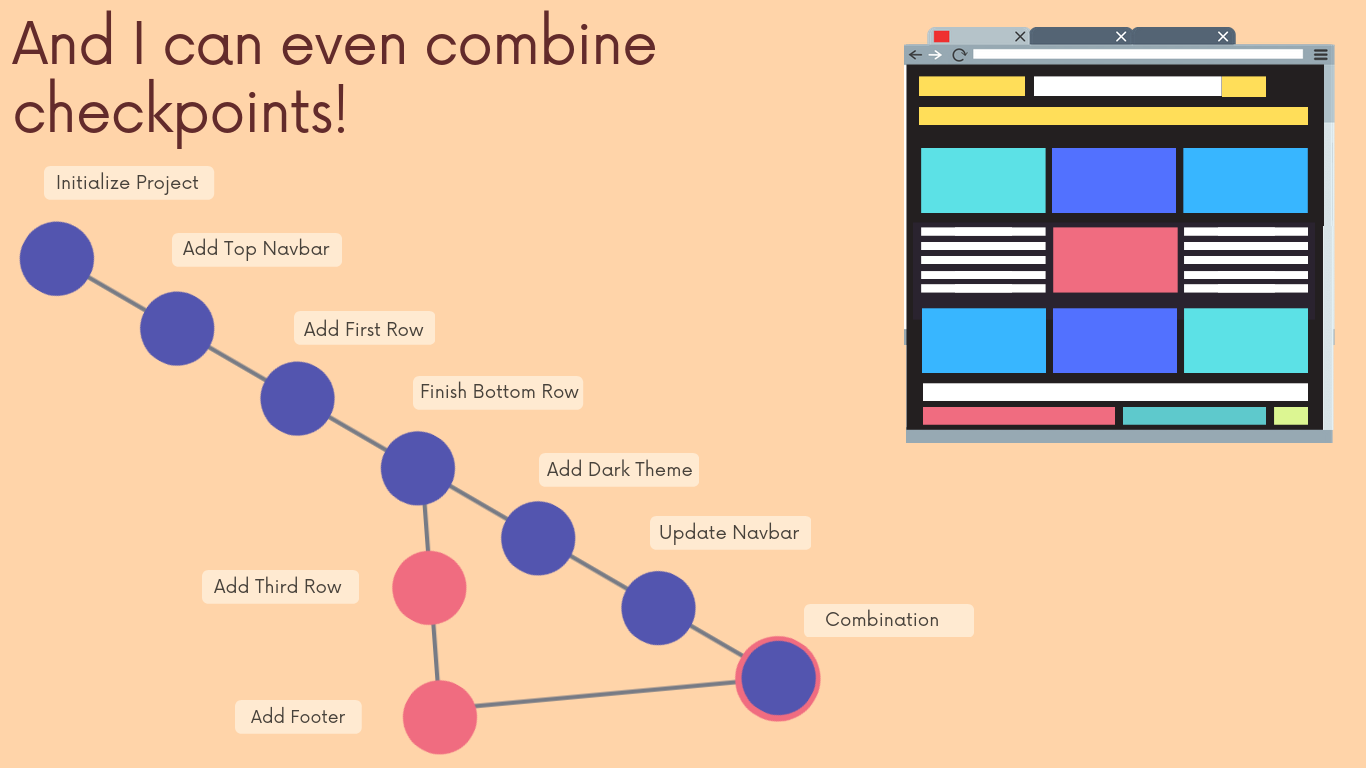
\includegraphics[width=2in]{screenshots/2022-06-26T21-27-54Z.png} 
	 \end{figure}

\end{itemize}
The big picture : \fbox{It's like check points in video games}


\section{Who uses it?}
\begin{itemize}
	\item Engineers \& Coders
	\item Tech-Adjacent Roles
	\item Governments 
	\item Scientist
	\item Writers
	\item Anyone (even musicians)
\end{itemize}


\section{Git vs. Github}
Git works locally on a machine whereas Github hosts Git repos in the cloud, makes it easy to collaborate. It is possible to upload local work to Github cloud.



\chapter{Installation \& Setup}


\section{Configuring Git Name \& Email}

Git needs to know who worked on what.

\begin{tcolorbox}[title=,colback=backcolour]
\begin{lstlisting}[language=bash]
git config --global user.name "Bob"
# Global means that the name will be consistent on all projects

git config --global user.email "bob@hello.com"

git config user.*
# To check current variable
\end{lstlisting}
\end{tcolorbox}


\section{Terminal Crash Course}

\subsection{Introduction}
\begin{itemize}
	\item \textbf{pwd} : prints out current directory path 
	\item \textbf{ls} + path : prints out files in a directory
	\item \textbf{open .} \textit{mac} or \textbf{start .} \textit{windows} opens up graphical file explorer in current dir 
\end{itemize}

\subsection{Creating Files \& Folders}
\begin{itemize}
	\item \textbf{mkdir} : makes a new directory (Supports multiple vars)
	\item \textbf{touch} file.ext : creates a file
\end{itemize}

\subsection{Deleting Files \& Folders}
\begin{itemize}
	\item \textbf{rm} to delete files, \textbf{rm -rf} to delete non-empty folder [recursive,force]  
\end{itemize}



\chapter{The Very Basics of Git}


\section{What's a Git Repo?}

A git repo = a workspace, on a machine, it will be linked to a folder


\section{Git Init and Git Status}
\begin{itemize}
	\item \textbf{git status} : gives current directory status 
	\item \textbf{git init} : current directory becomes a repo 
\end{itemize}


\section{Common Early Git Mistake}
\begin{itemize}
	\item Gits tracks a directory \textbf{and} all nested subdirectories
	\item \fbox{\warning DO NOT INIT A REPO INSIDE OF A REPO}
	\item Always check with git status first
\end{itemize}


\section{Committing Workflow Overview}

\begin{itemize}
	\item Commit $\equiv$ "a check point, snapshot in time" + a message
	\item A Commit groups changes on multiple files together $\not=$ saving a file
	\item It's a \textbf{multi steps} process
			\begin{figure}[H] 
	 		\centering 
	 		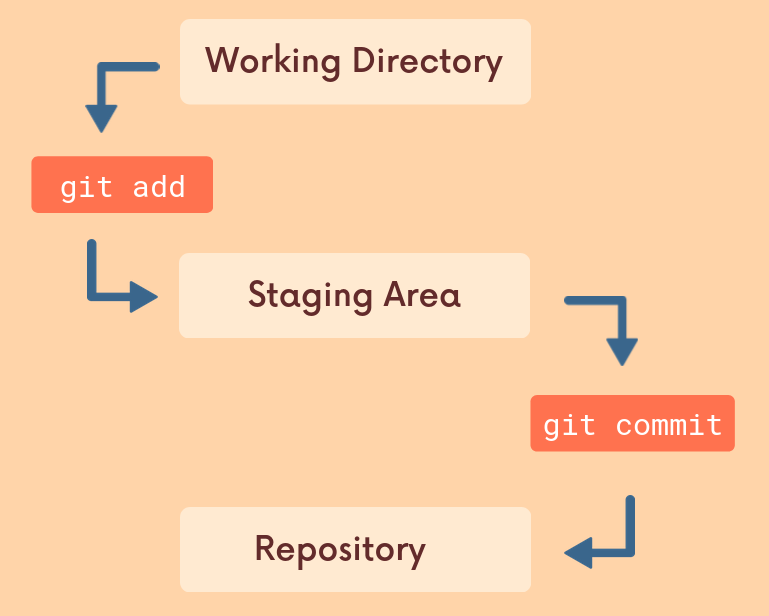
\includegraphics[width=2in]{screenshots/2022-06-26T23-07-02Z.png} 
		 \end{figure}
		\begin{itemize}
			\item Work on stuff
			\item Add Changes -- Group them together in preparation of committing.
				Very useful to select particular changes, group them, commit them
			\item Commit -- everything that was added

		\end{itemize}
\end{itemize}


\section{Staging Changes with Git Add}

\begin{itemize}
	\item \textbf{Working Directory} "the folder" 
	\item \textbf{Repository} git commit updates the ".git folder" 
	\item \textbf{Staging area} where we stage our changes before committing 
\end{itemize}

\begin{tcolorbox}[title=Adding,colback=backcolour]
\begin{lstlisting}[language=bash]
git add file1 file2
# add until ready to commit
git add .
# will stage all changes
git add Folder/
# will add everything inside a folder
\end{lstlisting}
\end{tcolorbox}


\section{Git Commit Command}

\begin{itemize}
	\item Git expects a message that \textbf{summarize} the changes in a commit 
	\item git commit will try to use the default editor in order to enter the message
\end{itemize}
\begin{tcolorbox}[title=Commit,colback=backcolour]
\begin{lstlisting}[language=bash]
git commit -m "my message"
# will do both commit and message tasks grouped
git commit -a -m "my message"
# will both add and commit
\end{lstlisting}
\end{tcolorbox}


\section{Git Log Command}

\begin{itemize}
	\item \textbf{git log} retrieves informations, logs of commits in a repo (author + date + message + hash)
\end{itemize}



\chapter{Committing in Details}


\section{Navigating the Git Documentation}
Link to the documentation\fbox{\href{https://www.git-scm.com}{git-scm.com}} 

Download the ebook


\section{Keeping our Commits Atomic}

\begin{itemize}
	\item \textbf{Atom} means a base unit : a single feature, change or fix. \textbf{each commit should be focussed on one single thing} 
\end{itemize}


\section{Commit Messages}

\begin{itemize}
	\item Documentation recommends to describe things in imperative mood as if we were giving orders to the codebase to change its behavior 
	\item Doesn't really matters but should be at least consistent
\end{itemize}


\section{Configuring Default Editor}
\begin{itemize}
	\item Git commit by itself (w/o -m), will open the default editor to write the message
\end{itemize}

\begin{tcolorbox}[title=Changing Editor,colback=backcolour]
\begin{lstlisting}[language=bash]
git config --global core.editor "nvim"
\end{lstlisting}
\end{tcolorbox}


\section{Closer Look at Git Log}
\begin{itemize}
	\item Commits message can be very long, while sometimes we only really need their hashes and a short message
\end{itemize}

\begin{tcolorbox}[title=Commit Formating,colback=backcolour]
\begin{lstlisting}[language=bash]
git log --pretty
git log --oneline 
# --oneline   is equiv   to --pretty-oneline --abbrev-commit
\end{lstlisting}
\end{tcolorbox}

\begin{itemize}
	\item This also means that the \textbf{first line} of each commit messages should already give enough informations. 
\end{itemize}


\section{Fixing Mistakes with Amend}

\begin{itemize}
	\item \textbf{Amending Commits} is usefull when forget to add to something a commit, or make a type in its message 
	\item It only works when the mistake has been made on the last commit 
	\item \textbf{--amend} will \textbf{redo} the last commit with the new files added  
\end{itemize}

\begin{tcolorbox}[title=Amending Commits,colback=backcolour]
\begin{lstlisting}[language=bash]
git commit -m '...'
git add forgotten_file
git commit --amend
# it will also open up the previous commit message in order to edit it
\end{lstlisting}
\end{tcolorbox}


\section{Ignoring Files w/ .gitignore}

\begin{itemize}
	\item \textbf{Ignoring Files} : is useful to list files that we never want to be tracked like passwd, log files, dependencies,... 
	\item \textbf{.gitignore} : Traditionally it has to be at the root of the repo. Following patterns will be used :
		\begin{itemize}
			\item \textit{filename} : will ignore a specific file 
			\item \textit{folder\_name/ } : will ignore an entire directory (the "/" is crucial)
			\item \textit{*.ext} : will ignore all files with \textit{.ext} extension
		\end{itemize}
	\item \textbf{.gitignore} Should also be add and committed 
	\item \fbox{gitignore.io} will list recommendation for things to ignore when using a specific programming language
\end{itemize}



\chapter{Working With Branches}


\section{Introducing Branches}
\begin{itemize}
	\item Every commit has a unique hash and reference at least one commit that came before it, a linear history
\begin{figure}[H] 
	 \centering 
	 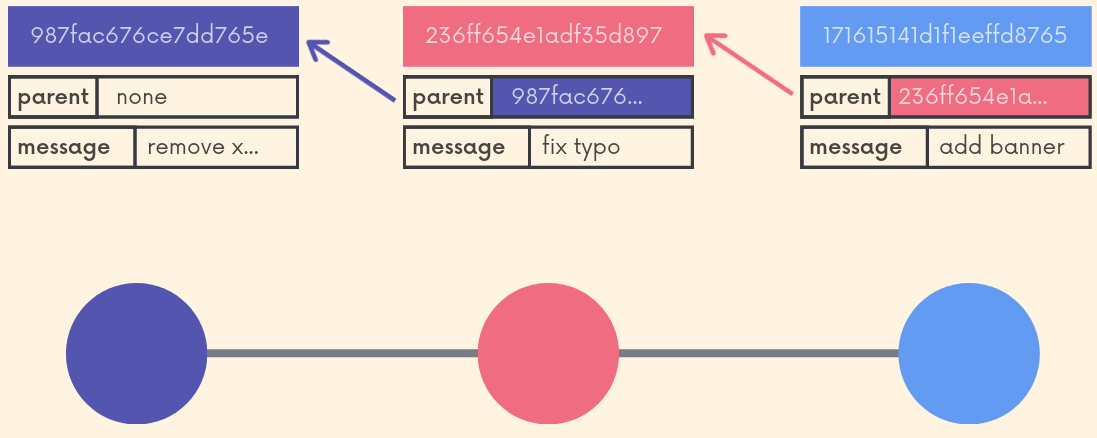
\includegraphics[width=4in]{screenshots/2022-06-28T00-13-49Z.png} 
\end{figure}
	\item \textbf{Context} : lot's of unrelated changes are made, in that case, a linear history will not suit our purposes.
		\begin{itemize}
			\item Those changes should happen in isolation 
		\end{itemize}
	\item \textbf{Branches} are like alternative timelines for a project. Allowing us to create separate context to try new things, work on multiple ideas in $ \| $  
	\item Changes on a branch \textbf{do not} affect other branches until we merge 
		\begin{figure}[H] 
	 \centering 
	 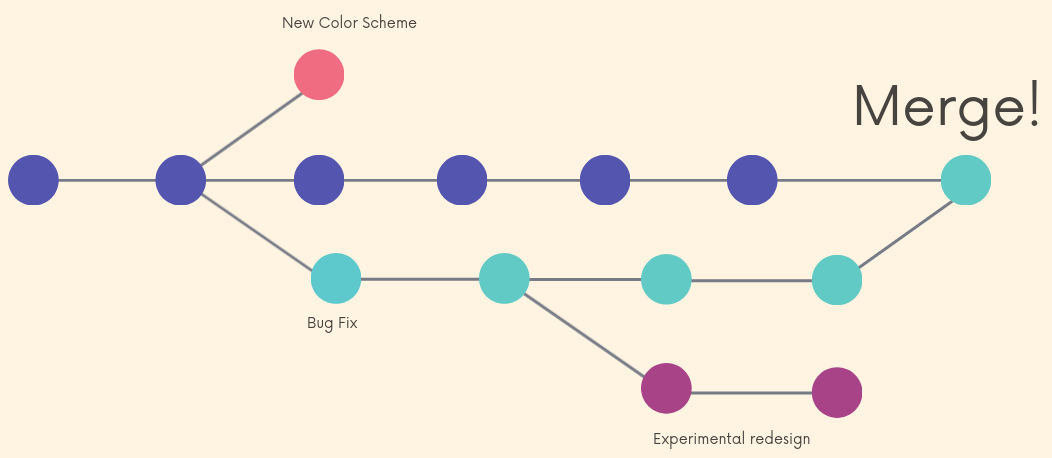
\includegraphics[width=4in]{screenshots/2022-06-28T00-24-00Z.png} 
 \end{figure}
\end{itemize}


\section{The Master Branch}

\begin{itemize}
	\item \textbf{The Master Branch} is the default branch name. Although it can be considered as the main definitive branch of a project, the one from which we do other test branches 
	\item Github has renamed default branch from Master $\mapsto$ Main
\end{itemize}

\begin{figure}[H] 
\centering 
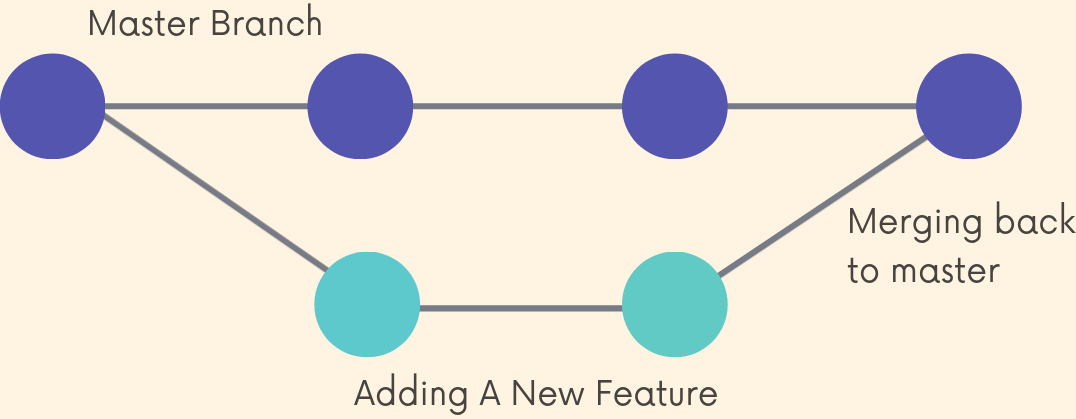
\includegraphics[width=4in]{screenshots/2022-06-28T00-30-17Z.png} 
\end{figure}


\section{What is HEAD?}

\begin{itemize}
	\item \textbf{HEAD} simply points to the current location in a repo, a particular branch release.
\end{itemize}


\section{Viewing All Branches with Git Branch}

\begin{tcolorbox}[colback=backcolour]
\begin{lstlisting}[language=bash]
git branch
\end{lstlisting}
\end{tcolorbox}


\section{Creating \& Switching Branches}
\begin{tcolorbox}[title=Creating Branches,colback=backcolour]
\begin{lstlisting}[language=bash]
git branch <branch_name>
\end{lstlisting}
\end{tcolorbox}
\begin{itemize}
	\item \warning The new branch will be based upon the current HEAD
	\item \warning The HEAD stays the same 
	\item The branch initially point to the previous one
\end{itemize}

\begin{tcolorbox}[title=Switching Branches,colback=backcolour]
\begin{lstlisting}[language=bash]
git switch <branch_name>
# Changes will occur immediately
git switch -c <branch_name>
# c for "create", makes it possible to create and switch at the same time
\end{lstlisting}
\end{tcolorbox}


\section{Git Checkout Vs. Git Switch}

\begin{itemize}
	\item Checkout as is does the same as switch but it can do a lot more than switch 
	\item \warning the equivalent of switch \textbf{-c} is checkout \textbf{-b} 
\end{itemize}


\section{Switching Branches With Unstaged Changes}

\begin{itemize}
	\item When a branch has work that has not been committed, switching to a $\not =$ branch \textbf{would make it lost}. 
	\item This is not a problem when the concerned file isn't in the other branch, this file will follow us in every branches we go to
\end{itemize}


\section{Deleting \& Renaming Branches}

\begin{tcolorbox}[title=Delete Branches,colback=backcolour]
\begin{lstlisting}[language=bash]
git branch -d <branch to delete>
\end{lstlisting}
\begin{itemize}
	\item Does not work if we currently are the said branch 
	\item Does not work if "not fully merged" $\rightarrow$ needs \textbf{-D} (forcing) 
\end{itemize}
\end{tcolorbox}

\begin{tcolorbox}[title=Rename Branches,colback=backcolour]
\begin{lstlisting}[language=bash]
git switch <to the branch we want to rename>
# we need to be on the said branch to rename it
git branch -m <name>
# m stands for move or rename
\end{lstlisting}
\end{tcolorbox}



\chapter{Merging Branches}


\section{Introduction to Merging}

\begin{itemize}
	\item Useful when we want to incorporate changes from one branch into another 
	\item \textbf{Common Workflow} : treat the Master branch as the most stable build, no experimentation allowed 
	\item To experiment we use a \textit{Feature Branch} 
\end{itemize}
Two important merging concepts :
\begin{enumerate}
	\item We merge branches, not specific commits 
	\item We always merge to the current HEAD branch
\end{enumerate}

\begin{tcolorbox}[title=Example,colback=backcolour]
\begin{lstlisting}[language=bash]
git switch master
git merge bugfix
# Here, Master simply caught up on the commits form Bugfix
# It is called a Fast Forward Merge
\end{lstlisting}
\end{tcolorbox}


\section{Performing A Fast Forward Merge}
\begin{enumerate}
	\item Switch to the destination branch 
	\item Then git merge
\end{enumerate}

\begin{itemize}
	\item Merging is easy when nothing as happened to the master branch since "splitting"
\end{itemize}


\section{Generating Merge Commits}
\begin{itemize}
	\item Not all merges are fast forward
\end{itemize}
\begin{figure}[H] 
	 \centering 
	 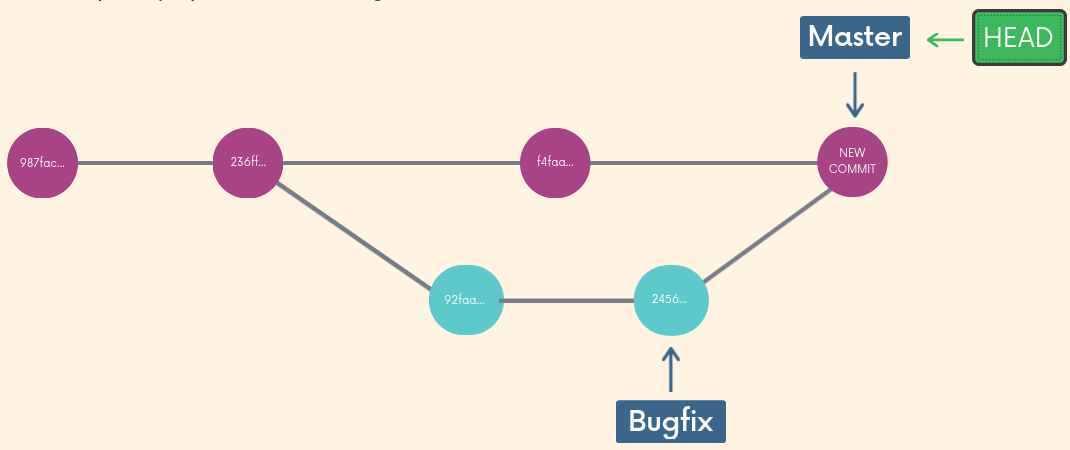
\includegraphics[width=4in]{screenshots/2022-07-01T21-35-16Z.png} 
	 \caption{Conflicting Work} 
 \end{figure}

 \begin{itemize}
	 \item If git is able to figure out how to combine the work by itself, then we simply end up with a \textbf{new commit}, the Master branch here doesn't just catch up, it generates a whole new commit with two parents
 \end{itemize}


 \section{Merge Conflicts}

 \begin{itemize}
 	\item We first need to fix conflicts and then commit the result
 \end{itemize}

 \begin{tcolorbox}[title=Conflicts Markers,colback=backcolour]
 \begin{lstlisting}[language=bash]
 <<<<<<<HEAD
 # Content of our current HEAD
 =======
 # Content from the branch we are trying to merge in
 >>>>>>>Bug-Fix
 \end{lstlisting}
 \end{tcolorbox}


 \section{Resolving Merge Conflicts}
 \begin{enumerate}
	 \item Open up the file(s) with merge conflicts 
	 \item Edit them to remove conflicts. Decide which branch's content you want to keep / keep both 
	 \item Remove "conflicts markers" in the document 
	 \item Add changes and commit
 \end{enumerate}



\chapter{Comparing Changes With Git Diff}


\section{Introducing The Git Diff Command}

\begin{itemize}
	\item \textbf{git diff} is about showing changes, get a picture
		\begin{itemize}
			\item Between commits, branches, files, working directory
		\end{itemize}
	\item By default it lists all the \textbf{unstaged} changes only
\end{itemize}


\section{How To Read Git Diffs}

\begin{tcolorbox}[colback=backcolour]
\begin{lstlisting}[language=bash]
diff --git <first-file> <second-file>
index # file metadata
--- <old-file>
+++ <new-file>
# @@ chunks header @@ 
# chunk...
\end{lstlisting}
\end{tcolorbox}

\begin{itemize}
	\item \textbf{Chunks} are portions of files containing modifications and context
	\item \textbf{Chunks Headers} @@ -file a , +file b @@, the \textbf{numbers} in between represent how many lines have been extracted
\end{itemize}


\section{Viewing Working Directory Changes}

\begin{itemize}
	\item \textbf{git diff HEAD} will list \textbf{all} changes in the working tree since last \textbf{commit} / HEAD
\end{itemize}


\section{Viewing Staged Changes}

\begin{itemize}
	\item git diff \textbf{--staged or --cached} will list changes between staging area and last commit, shows what will be included in the next commit 
\end{itemize}


\section{Diffing Specific Files}

\begin{itemize}
	\item git diff \textbf{[method] [filename(s)]} 
\end{itemize}


\section{Comparing Changes Accross Branches}

\begin{itemize}
	\item git diff \textit{branch1\textbf{..}branch2} 
	\item "\textbf{..}" can be replaced by a space
\end{itemize}


\section{Comparing Changes Across Commits}

\begin{itemize}
	\item git diff \textit{hash1\textbf{..}hash2} 
\end{itemize}


\section{Remark}

\begin{itemize}
	\item \warning git diff methods and arguments can all be combined
\end{itemize}



\chapter{The Ins and Outs of Git Stashing}


\section{Why We Need Stashing}
\begin{itemize}
	\item What happens when i have uncommitted changes on one branch and i try to switch to another one ?
			\begin{enumerate}
				\item The changes will just come with us 
				\item Git won't let us switch if it detects potential \textbf{conflicts}
			\end{enumerate}
\end{itemize}


\section{Git Stash Save \& Pop}

\begin{itemize}
	\item \textbf{git stash} or git stash \textbf{save} : will take all uncommitted changes and stash them, reverting changes in our working copy 
	\item \textbf{git stash pop} to re-apply them to our working copy and empty the stash
\end{itemize}


\section{Git Stash Apply}

\begin{itemize}
	\item \textbf{git stash apply} : will take everything in the stash and apply it, just like \textbf{pop} but it stays in the stash afterwards
\end{itemize}


\section{Working With Multiple Stashes}

\begin{itemize}
	\item We can make a \textbf{stack} of stashes, kept in the order we make them 
	\item \textbf{git stash list} to view all stashes 
	\item To apply a \textbf{specific stash}, we use the given \textit{stash-id} : \textbf{stash@{i}}  
\end{itemize}


\section{Dropping \& Clearing the Stash}

\begin{itemize}
	\item \textbf{git stash drop stash@{i}} 
	\item \textbf{git stash clear} to remove everything from the stash
\end{itemize}



\chapter{Undoing Changes \& Time Traveling}


\section{Checking Out Commits}

\begin{itemize}
	\item \textbf{git checkout} can create branches, switch to new branches, restore files and undo history 
	\item git checkout \textbf{<commit-hash>} to view a previous commit
		\begin{itemize}
			\item \warning We just need the first \textbf{7} digits of it 
			\item Executing this command will bring us (the HEAD) back in time 
			\item Make sure to not have unstaged changes
		\end{itemize}
	\item HEAD usually refers to a branch, \textbf{not} a specific commit
\end{itemize}

\begin{figure}[H] 
	 \centering 
	 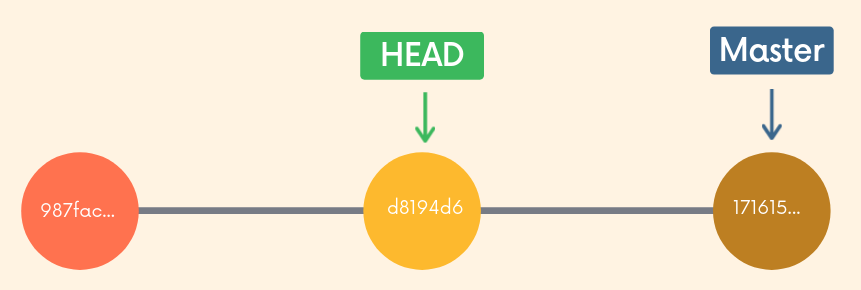
\includegraphics[width=2.5in]{screenshots/2022-07-06T18-51-35Z.png} 
 \end{figure}


\section{Re-Attaching Our Detached HEAD}

\begin{itemize}
	\item Options when we have a detached HEAD
		\begin{enumerate}
			\item Stay in it and examine contents of old commit : view the files,.. 
			\item Leave and go back to wherever we were before : \textbf{Re-attach} the HEAD 
			\item \textbf{Create} a new branch and \textbf{switch} to it. You can now \textbf{make} and \textbf{save} changes, HEAD is no longer detached
		\end{enumerate}
\end{itemize}


\section{Referencing Commits Relative to HEAD}

\begin{itemize}
	\item git checkout \textbf{HEAD$ \sim $i}
		\begin{itemize}
			\item i = 1 refers to the commit before HEAD (parent)
			\item i = 2 refers to 2 commits before HEAD (grandparent)..
		\end{itemize}
	\item git \textbf{switch -} to switch to the branch we were on last. Alternatively, just switch to the branch 
\end{itemize}


\section{Discarding Changes With Git Checkout}

\begin{itemize}
	\item To revert the file back to whatever it looked like when you last committed (specificaly \textbf{where HEAD is referencing}), we use :
		\begin{itemize}
			\item git checkout \textbf{HEAD filename(s)} 
			\item git checkout \textbf{- - filename(s)} \textit{is a shorter version}
		\end{itemize}
\end{itemize}


\section{Un-Modifying With Git Restore}

\begin{itemize}
	\item git checkout does a lot of things so git restore was introduced alongside git switch 
	\item \textbf{git restore filename} : will revert back to where HEAD is pointing, trashing all uncommited changes 
	\item git restore \textbf{- -source HEAD$\sim$i filename} : to use something else than HEAD as the source 
	\item It does not do a time travel! It only modifies the file(s)
\end{itemize}


\section{Unstaging Files With Git Restore}

\begin{itemize}
	\item git restore \textbf{- -staged} filename 
\end{itemize}


\section{Undoing Commits With Git Reset}

\begin{itemize}
	\item Situation : we made some commits on the wrong branch 
	\item git \textbf{reset <commit-hash>} : will reset repo back to a specific commit. The commits are done \textbf{but} \warning the changes are still in our working directory 
	\item Now we can switch branch and add a commit with the changes 
	\item If we want to remove commits \textbf{AND} changes, we use the \textbf{- -hard} option
\end{itemize}

\begin{tcolorbox}[title=Example,colback=backcolour]
\begin{lstlisting}[language=bash]
git reset --hard HEAD~1
\end{lstlisting}
\end{tcolorbox}


\section{Reverting Commits With Git Revert}

\begin{itemize}
	\item \textbf{git reset} actually moves the branch point backwards, eliminating commits \textit{while} \textbf{git revert} creates a brand new commit 
	\item Syntax : \textbf{git revert <commit-hash>} 
	\item Which one should we use ?
		\begin{itemize}
			\item If we want to reverse commits that have been \textbf{shared} with other people, we should use \textbf{revert}, although it could lead to conflicts 
			\item Otherwise we could use \textbf{reset} 
		\end{itemize}
\end{itemize}



\chapter{Github : The Basics}


\section{What Does Github Do For Us}

\begin{itemize}
	\item Github helps people share and collaborate on repos 
	\item Other options : [Gitlab, BitBucket, Guerrit]
\end{itemize}


\section{Why We Should Use It}

\begin{itemize}
	\item Employers often look at github profiles
\end{itemize}


\section{Cloning Repos With Git Clone}

\begin{itemize}
	\item \textbf{git clone <url>} get's a local copy of an existing repository, it will initialize itself and give access to the full history 
	\item \warning Make sure not to be in a existing repo 
\end{itemize}


\section{Github Setup : SSH Config}

\begin{itemize}
	\item \textbf{SSH Keys} allows to connect to Github without needing to enter credentials 
	\item \href{https://docs.github.com/en/authentication/connecting-to-github-with-ssh/generating-a-new-ssh-key-and-adding-it-to-the-ssh-agent}{Link to configure ssh keys} 
\end{itemize}


\section{How Do I Get My Code On Github}

\begin{itemize}
	\item \textbf{Options :}
		\begin{enumerate}
			\item Existing Repo
				\begin{enumerate}
					\item Create a new empty repo on Github 
					\item Connect your local repo (add a remote) 
					\item Push up your changes
				\end{enumerate}
			\item Start from scratch \label{scratch}
				\begin{enumerate}
					\item Create a brand new repo on Github 
					\item Clone it down to your machine 
					\item Do some work 
					\item Push it up
				\end{enumerate}
		\end{enumerate}
\end{itemize}


\section{Crash Course On Git Remotes}

\begin{itemize}
	\item Before pushing, we need to tell git about our remote repo on Github, setup a \textbf{destination} 
	\item Each remote is simply a URL where a hosted repo lives 
	\item \textbf{git remote \textit{-v}} to display a list of remotes (\textit{v stands for verbose}) 
	\item \textbf{git remote add <name> <url>} to add a new remote
		\begin{itemize}
			\item The \textbf{name} \textit{origin} is conventionally the default remote name 
			\item \warning url is in the form of git@github.com:Username/repo.git
		\end{itemize}
	\item git remote \textbf{rename <old> <new>} 
	\item git remote \textbf{remove <name>}  
\end{itemize}


\section{Introducing Git Push}

\begin{itemize}
	\item \textbf{git push <remote> <branch>} will push our work to the online repo 
	\item \warning for Github, we could rename branch "master" to "main" before pushing with : \textbf{git branch -M main} 
\end{itemize}


\section{A Closer Look At Git Push}

\begin{itemize}
	\item There is a distinction between local and online branches 
	\item Usually we want to connect local and online master branches 
	\item To push a local branch "A" to an online branch "B" we can do : \textbf{git push <remote> <local-branch>:<remote-branch>} 
\end{itemize}


\section{Meaning of Git Push -u}

\begin{itemize}
	\item \textbf{git push -u <remote> <branch>} where \textbf{u} stands for "upstream", acts like a connection pointing towards a remote branch. It will take our current local branch and link it to the <specified> online branch
\end{itemize}

\begin{figure}[H] 
	 \centering 
	 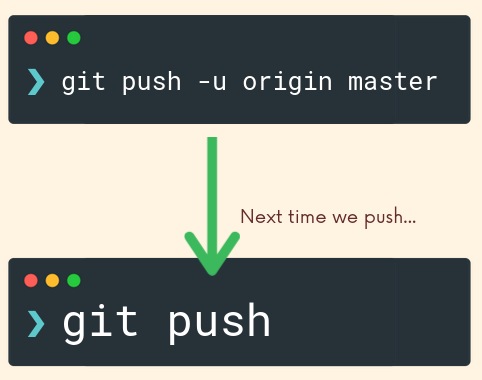
\includegraphics[width=1.7in]{screenshots/2022-07-07T20-52-46Z.png} 
	 \caption{push will now refer to the link we made with \textbf{-u}} 
 \end{figure}

 \begin{tcolorbox}[title=Playing with branches,colback=backcolour]
 \begin{lstlisting}[language=bash]
 git push -u origin dogs:cats
 # for the future, this dogs branch will be linked to the up to remote cats branch online. The dogs branch will also have an upstream referring to the cats branch
 \end{lstlisting}
 \end{tcolorbox}


\section{The Other Github Workflow : Cloning First [\ref{scratch}]}

\begin{itemize}
	\item Cloning it first will automatically initialize remote : \textbf{origin}
\end{itemize}



\chapter{Fetching \& Pulling}


\section{What Are Remote Tracking Branches?}

\begin{itemize}
	\item When we clone a repo, the repo gets copied on my machine with all its commits. But there's actually \textbf{2} branches references :
		\begin{itemize}
			\item The regular branch reference that i can move around 
			\item The other one is a \textbf{Remote Tracking Branch}, a reference to the state of the master branch on the remote. I \textbf{cannot} move it
		\end{itemize}
\end{itemize}

\begin{figure}[H] 
	 \centering 
	 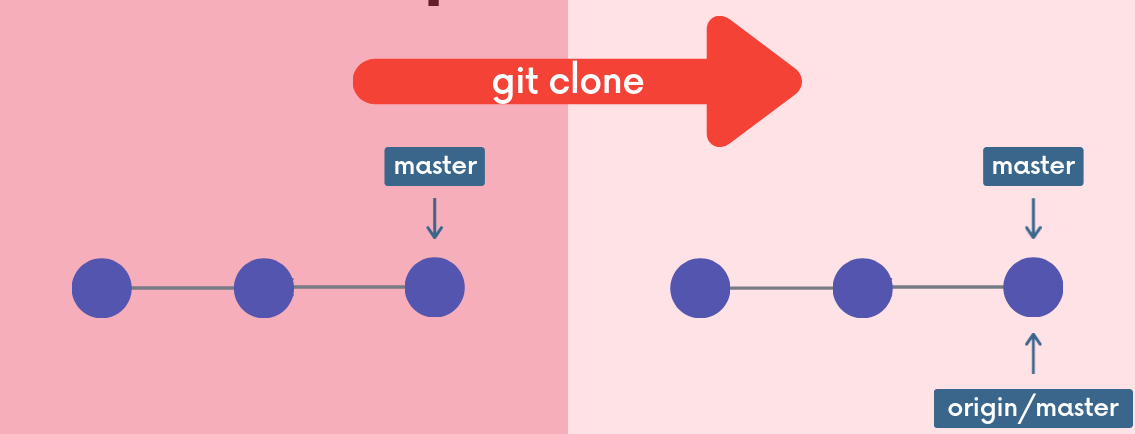
\includegraphics[width=2in]{screenshots/2022-07-08T10-45-10Z.png} 
\end{figure}

\begin{itemize}
	\item "At the time you last communicated with this remote repo, here is what branch A was pointing" 
	\item Following the pattern \textbf{<remote>/<branch>} 
	\item \textbf{git branch -r} to view remote branches our local repo knows about
\end{itemize}


\section{Checking Out Remote Tracking Branches}

\begin{tcolorbox}[title=After some work on main branch,colback=backcolour]
\begin{lstlisting}[language=bash]
Your branch is ahead of 'origin/main' by ... commits.
# the reference stood the same
\end{lstlisting}
\end{tcolorbox}

\begin{itemize}
	\item To know how was the repo before my modifications : \textbf{git checkout origin/master} 
\end{itemize}


\section{Working With Remote Branches}

\begin{itemize}
	\item When i clone a repo, i only end up with the \textbf{default branch}. But i still get the remotes for all those other branches 
	\item There's a relationship between a workspace branch and a remote branch
		\begin{itemize}
			\item By default, the master branch is connected to the origin/master 
		\end{itemize}
	\item How do i work on a non-default branch
		\begin{itemize}
			\item I can git \textbf{checkout} origin/branch 
			\item $\diamond$ But i actually want to get a \textbf{connection} with \textbf{git switch <remote-branch-name>} it will make me a local \textit{<name>} branch and set it up to track the remote branch origin/\textit{<name>}
		\end{itemize}
\end{itemize}


\section{Git Fetch: The Basics}

\begin{figure}[H] 
	 \centering 
	 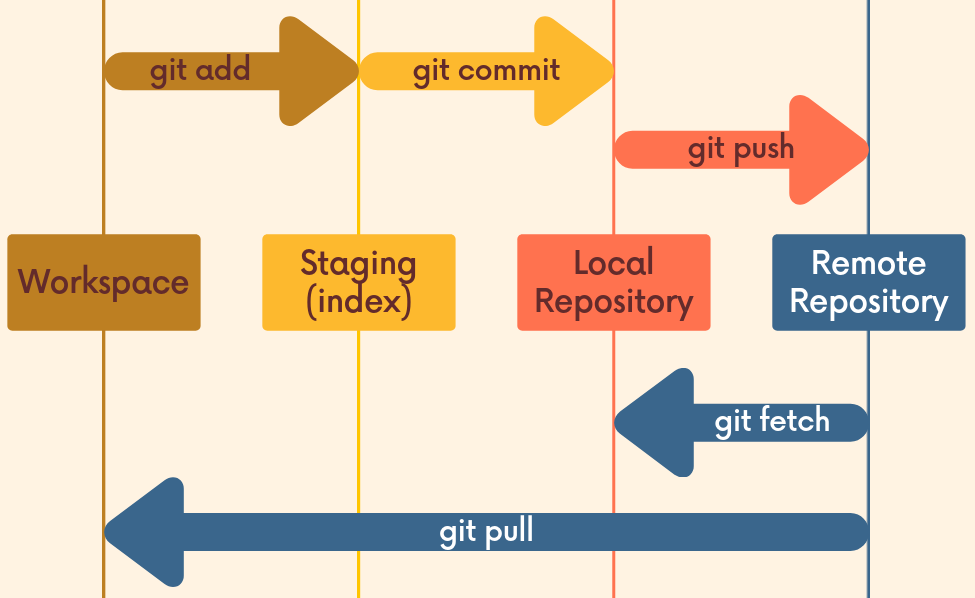
\includegraphics[width=3in]{screenshots/2022-07-08T16-53-13Z.png} 
 \end{figure}

\begin{itemize}
	\item $\diamond$ \textbf{git fetch <remote> <branch>} will take remote changes and bring them down to the local repo, the default \textbf{<remote>} is \textbf{origin}, \textbf{<branch>} is \textbf{optional}
	\item "Please go and get the latest info from github but don't screw up my working directory"
\end{itemize}

\begin{figure}[H] 
	 \centering 
	 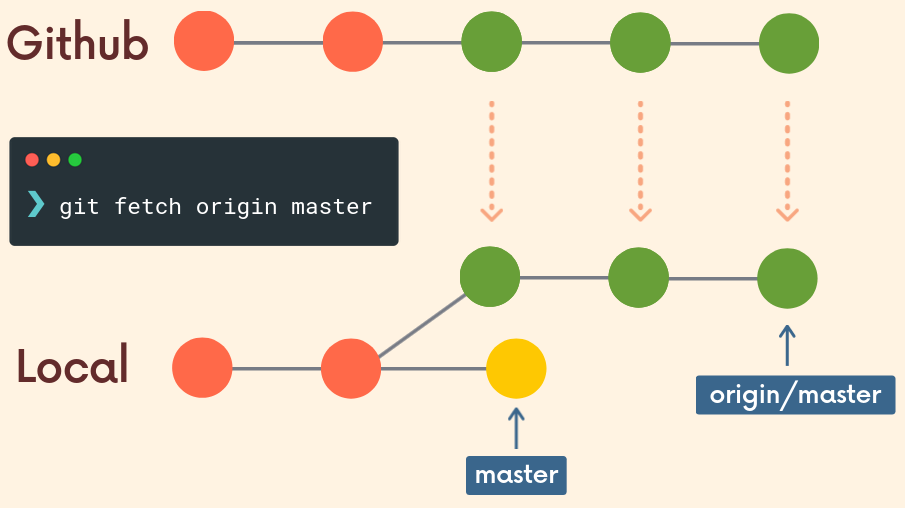
\includegraphics[width=2.5in]{screenshots/2022-07-08T16-59-32Z.png} 
 \end{figure}

 
\begin{itemize}
	\item My branch will be left \textbf{untouched}, i can then checkout \textbf{remote/branch}
\end{itemize}


\section{Git Pull: The Basics}

\begin{itemize}
	\item Unlike fetch, pull actually updates our HEAD branch 
	\item "Go and download data online and immediately update my local repo with those changes" 
	\item git pull = git fetch + git merge 
	\item $\diamond$ \textbf{git pull <remote> <branch>} to pull, \warning whatever branch we run it from is where the changes will be merged into 
	\item A good practice is to always pull down changes \textbf{before} pushing 
	\item \textbf{An easier syntax} : \textbf{git pull} will default to the origin remote and to whatever branch is configured to be tracked for our current branch 
	\item Pulling is \textbf{not} recommended when we have uncommitted changes
\end{itemize}


\chapter{Github Grab Bag: Odds \& Ends}

\section{Adding Github Collaborators}

\begin{itemize}
	\item Allowing other users to \textbf{push} to the repo as well as seeing it, but they \textbf{cannot access settings} 
	\item Repo $\rightarrow$ Settings $\rightarrow$ Manage access
\end{itemize}

\section{READMEs}

\begin{itemize}
	\item It is used to tell important informations about the repo such as :
		\begin{itemize}
			\item What the project does 
			\item How to run it 
			\item Why it's noteworthy 
			\item Who maintains it
		\end{itemize}
	\item Placed at the root of the repo, Github will automatically display it
\end{itemize}

\section{Markdown Crash Course}

\begin{itemize}
	\item Markdown is an html converter 
	\item > blockquotes can be nested 
	\item Inline code with `..` 
	\item Block code with ```language \textbackslash n ... \textbackslash n ``` 
	\item Links : [link text](url)
	\item Images : \textbf{!} [link text](url)
\end{itemize}


\section{Creating Github Gists}

\begin{itemize}
	\item Github Gists are a simple way to share code snippets, while being simpler, they offer far less features than typical repos, it's a bit like \textbf{pastebin} 
	\item gist.github.com 
	\item A lot of Gists are \textbf{markdown}
\end{itemize}


\section{Github Pages}

\begin{itemize}
	\item Github pages allows to create websites simply by pushing our code 
	\item It only allows static sites, it only supports html/css/js 
	\item There are two types of gh pages :
		\begin{itemize}
			\item \textbf{User Site} : one per account, where we should host a portfolio
			\item \textbf{Project Sites} : one for each repo
		\end{itemize}
	\item Create page : repo $\rightarrow$ settings $\rightarrow$ gh pages, we could set our repo to have a specific branch for the website containing \textbf{index.html}, the conventional name for that branch is \textbf{gh-pages}  
\end{itemize}


\chapter{Git Collaboration Workflows}

\section{The Pitfalls Of A Centralized Workflow}

\begin{itemize}
	\item The \textbf{easiest} collaborative workflow, to have everyone work on a single branch, good for little teams but the worst in general 
	\item Problems : lots of time spent resolving conflicts and merging code, can't work on anything without disturbing the main codebase
\end{itemize}

\section{The All-Important Feature Branch Workflow}

\begin{itemize}
	\item \textbf{Nobody} works on the main branch, main is the official project history 
	\item Teammates can collaborate on a single feature without polluting main so no broken code on main 
	\item We push branches up, and then merge with main
\end{itemize}

\section{Merging Feature Branches}

\begin{itemize}
	\item Features have to be merged back into main at some point, a couple of ways to achieve that :
		\begin{enumerate}
			\item Merge at will, without asking 
			\item Chat with the team 
			\item \textbf{Pull Requests!} 
		\end{enumerate}
\end{itemize}

\section{Introducing Pull Requests}

\begin{itemize}
	\item Pull Requests are a \textbf{feature} built in services such as Github, \textbf{not native to git} 
	\item It allows to alert on work to be reviewed, accepted or rejected, as well as discussing on specific commits 
	\item Describing the workflow :
		\begin{enumerate}
			\item Do some work locally on a feature branch 
			\item Push up the feature branch on Github 
			\item Open a pull requests using that feature branch 
			\item Wait for the PR to be approved and merged, start a discussion
		\end{enumerate}
\end{itemize}

\section{Making A Pull Request}

\begin{itemize}
	\item We can first \textbf{compare changes} which will tell if it would be able to merge easily 
	\item The branch to merge can still evolute before being merged or rejected 
	\item It could be a not \textbf{fast-forward} merge
\end{itemize}

\section{Resolving PR Merging Conflicts}

\begin{tcolorbox}[title=Checking out via command line,colback=backcolour]
\begin{lstlisting}[language=bash]
# Step 1: From your project repository, bring the changes and test
git fetch origin
git checkout -b branch origin/branch || git switch branch
git merge main
# We are now sure that this version can be applied to main without conflicts
# Step 2: Merge the changes and update on Github
git checkout main || git switch main
git merge --no-ff branch
# --no-ff to force a commit, keep an history
git push origin main
# Github will then automatically close the PR
\end{lstlisting}
\end{tcolorbox}

\section{Configuring Branch Protection Rules}

\begin{itemize}
	\item Settings $\rightarrow$ Branches $\rightarrow$ Branch protection rules 
	\item We can restrain branch a name pattern 
\end{itemize}

\section{Introducing Forking}

\begin{itemize}
	\item \textbf{The fork and Clone workflow} : Instead of one big centralized repo, every dev has their own one in addition to a main one. Devs make changes and push their own forks before making PR's 
	\item Common for large projects with few maintainers and thousands of contributors 
	\item Forking : allows to create personal copies of repos : "Forks of the original", it is a Github specific feature
\end{itemize}

\section{The Fork And Clone Workflow}

\begin{itemize}
	\item Github is automatically asking if we want to make a PR with the changes of my fork to the main one 
\end{itemize}

\begin{enumerate}
	\item Fork the official repo 
	\item Clone it to my machine, giving me the origin remote to my fork 
	\item Set up another remote, upstream between my local machine and the official repo, so i can fetch and pull from the original : \textbf{git remote add upstream https://github.com/User/repo.git} 
	\item Do some work (normally, we work on a seperate branch)
	\item Push to origin 
	\item Open PR
\end{enumerate}
\begin{figure}[H] 
	 \centering 
	 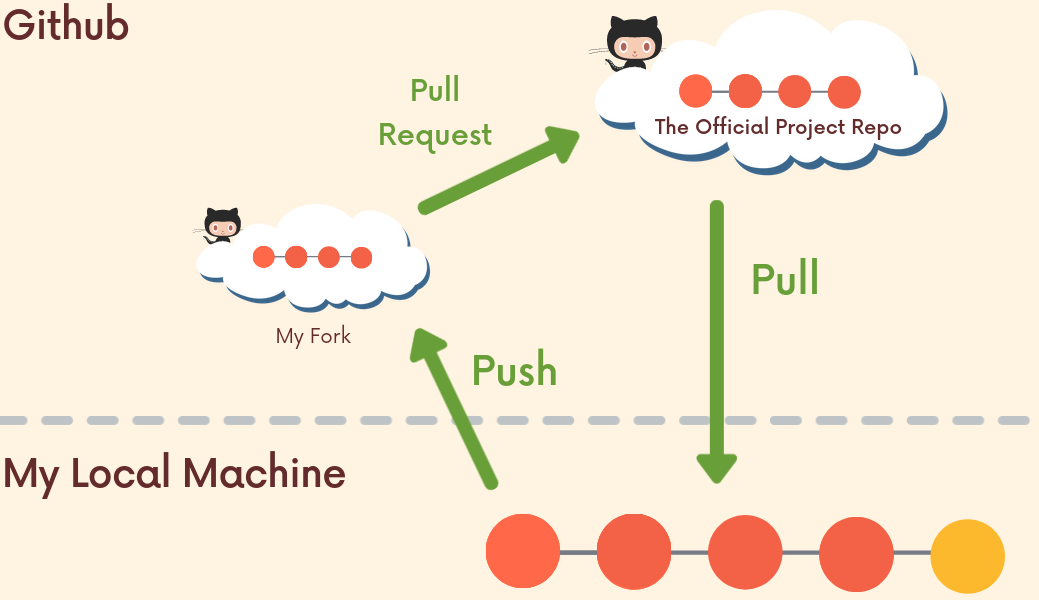
\includegraphics[width=2.5in]{screenshots/2022-07-09T19-19-34Z.png} 
 \end{figure}

\chapter{Git Rebase}

\section{What Is It?}

\begin{itemize}
	\item Two ways Rebasing is used :
		\begin{itemize}
			\item As an alternative to merging 
			\item As a cleanup tool
		\end{itemize}
	\item With merging, the history get's muddy
\end{itemize}
\begin{figure}[H] 
	 \centering 
	 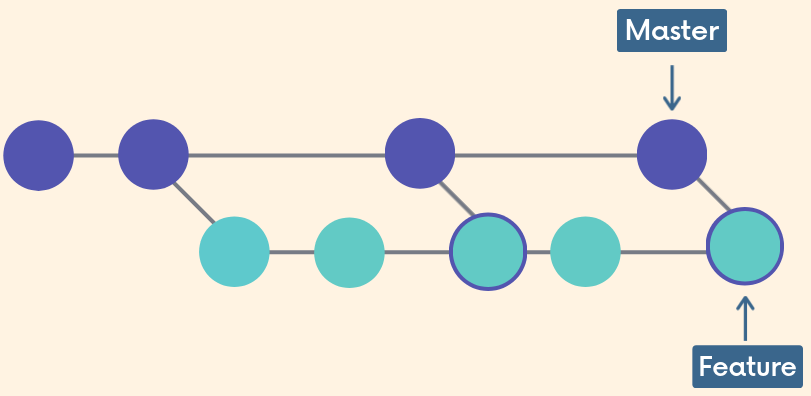
\includegraphics[width=2in]{screenshots/2022-07-09T20-15-48Z.png} 
 \end{figure}

\begin{itemize}
	\item If instead, we \textbf{rebase} the feature branch onto the main branch, this moves the entire feature branch so that it \textbf{begins} at the tip of the main branch. All the work is there but the history has been rewritten 
	\item Rebasing re-write history by \textbf{creating new commits} for each of the original feature branch commits. We are coming up with a \textbf{new base for our feature branch}. It will contain all the commits from master and feature  
	\item We rebase with \textbf{git switch feature} \&\& \textbf{git rebase main} 
\begin{figure}[H] 
	 \centering 
	 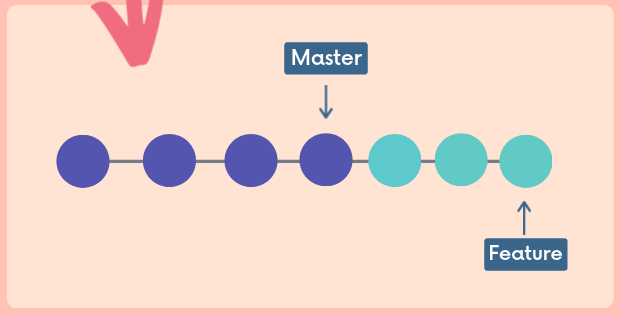
\includegraphics[width=2in]{screenshots/2022-07-09T20-22-40Z.png} 
\end{figure}

\begin{itemize}
	\item Both rebasing alone and merging with rebase after, works
\end{itemize}

\end{itemize}

\section{The Golden Rule: When Not To Rebase}

\begin{itemize}
	\item Because we are re-writing history : \warning \textbf{Never} Rebase commits that have been shared with others. If you have already pushed commits to github, \textbf{do not} rebase them unless sure that no one is using those commits
\end{itemize}

\section{Handling Conflicts \& Rebasing}
\begin{itemize}
	\item It pauses halfway through and let us either remove conflicts add them and continue \textbf{or} abort
\end{itemize}



\chapter{Cleaning Up History With Interactive Rebase}


\section{Interactive Rebase}

\begin{itemize}
	\item Rebase as a \textbf{cleanup tool}, we use \textbf{-i} to enter interactive mode, which allows us to edit, drop commits, add files, etc. We also need to specify how far we want to rewrite commits 
	\item \textbf{git rebase -i HEAD~4} 
	\item We are rebasing a series of commits onto the HEAD they are currently based on, applying rebase on it's own branch
\end{itemize}

\begin{enumerate}
	\item Create a new branch 
	\item \textbf{git rebase -i HEAD$\sim$i} 
	\item Opens up an editor with a list of commits with commands in front, \textbf{common commands} :
		\begin{itemize}
			\item \warning only change commands !
			\item \textbf{pick} : use the commit 
			\item \textbf{reword} : edit commit message 
			\item \textbf{edit} : use commit, but stop for amending 
			\item \textbf{fixup} : use commit, contents but meld it into previous commit and discard commit message 
			\item \textbf{drop} : remove commit, and contents will be done
		\end{itemize}
	%\item git switch main
\end{enumerate}

\chapter{Git Tags}

\section{The Idea Between Git Tags}

\begin{itemize}
	\item Tags refers to particular points in git history, it is like branch references that remains the same, just a label for a commit 
	\item Most often used to mark releases (\textit{v1.1.2,..}) 
\end{itemize}

\begin{figure}[H] 
	 \centering 
	 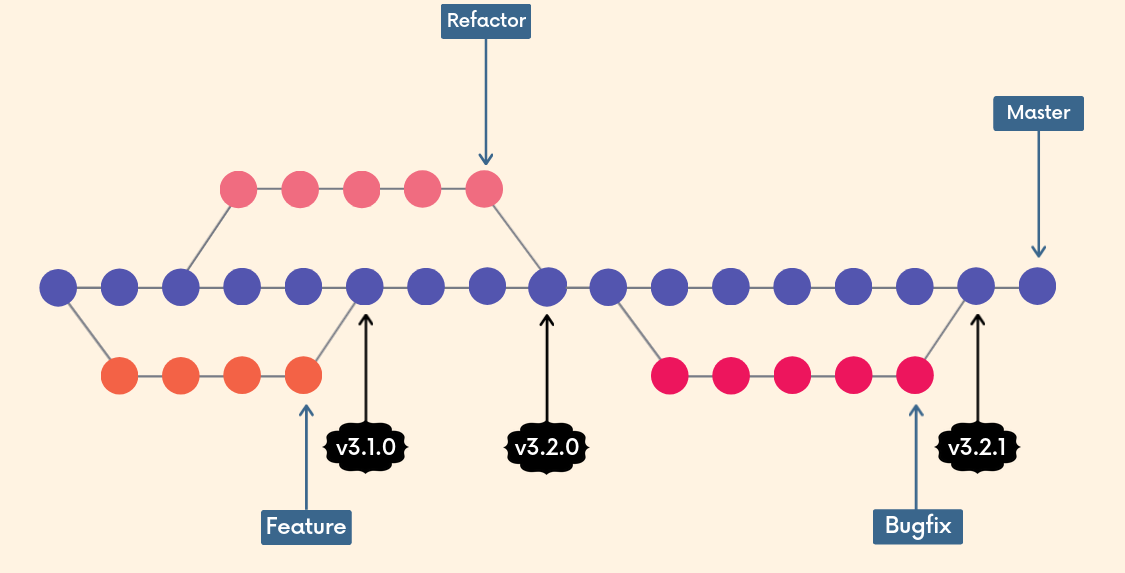
\includegraphics[width=3in]{screenshots/2022-07-10T01-23-06Z.png} 
\end{figure}

\begin{itemize}
	\item The 2 types of tags :
		\begin{itemize}
			\item \textbf{lightweight}, just name / label 
			\item \textbf{annotated}, store extra meta data like author's name, email, the date, message
		\end{itemize}
\end{itemize}

\section{Semantic Versioning}

\begin{itemize}
	\item A protocol that defines the meaning of \textit{2.4.1} $\rightarrow$ see \textbf{semver.org} 
	\item major-release.minor-release.patch-release, starts at \textbf{1.0.0} 
		\begin{itemize}
			\item \textbf{Patch} releases do not contain features or significant changes, typically : bug fixes and other changes that do not impact how the code is used 
			\item \textbf{Minor} releases do contain new \textbf{optional} features, the project is \textbf{still backward compatible} : should not force users to rewrite their code. We then have to \textbf{reset} patch number to 0
		\end{itemize}
\end{itemize}

\section{Viewing Tags}

\begin{itemize}
	\item \textbf{git tag} by default, will list all the tags in the current directory 
	\item \textbf{git tag -l "*pattern*"} will list all the tags that have "pattern" in their name, * means any character
\end{itemize}

\section{Comparing Tags With Git Diff}

\begin{itemize}
	\item \textbf{git checkout <tag>} $\rightarrow$ detached HEAD, i could then create a branch and start working from there
\end{itemize}

\begin{tcolorbox}[title=Diffing between two tags,colback=backcolour]
\begin{lstlisting}[language=bash]
git diff v17.0.0 v17.0.1
\end{lstlisting}
\end{tcolorbox}

\section{Creating Lightweight Tags}

\begin{itemize}
	\item \textbf{git tag <tagname>} will default to where the commit HEAD is pointing to
\end{itemize}

\section{Creating Annotated Tags}

\begin{itemize}
	\item \textbf{git tag -a <tagname>} will open default text editor 
	\item To see a tag's metadata : \textbf{git show <tagname>} 
\end{itemize}


\section{Tagging Previous Commits}

\begin{itemize}
	\item \textbf{git tag \textit{-a} <tagname> <commit-hash>} 
\end{itemize}

\section{Replacing Tags With Force}

\begin{itemize}
	\item When the tag does not refer to the good commit, we can use \textbf{git tag <tagname> <commit-hash> -f} 
\end{itemize}

\section{Deleting Tags}

\begin{itemize}
	\item \textbf{git tag -d <tagname>} 
\end{itemize}

\section{! Pushing Tags}

\begin{itemize}
	\item \warning by default \textbf{git push} will not include tags, to include them : \textbf{git push - -tags} will push all the tags, to include a single tag, use \textbf{git push <remote> <tag>} 
\end{itemize}


\chapter{Git Behind The Scenes: Hashing \& Objects}

\section{Working With The Local Config file}

\begin{itemize}
	\item Config file includes global settings like email, name, global or per repo 
	\item Editing .git/config in a repo will only change things in a specific repo 
	\item \textbf{git config} will apply changes globally, but \textit{--local} will allow to do it locally
\end{itemize}

\section{Inside Git: The Refs Directory}

\begin{itemize}
	\item \textbf{heads} contains branches files with the commit they are referring to
	\item \textbf{remotes} the same concept as heads
	\item \textbf{tags} 
\end{itemize}


\section{Objects Folder}

\begin{itemize}
	\item The objects folder is where git stores compressed and encrypted objects :
		\begin{itemize}
			\item commit, tree, blob, annotated tag
		\end{itemize}
\end{itemize}

\section{Crash Course On Hashing Functions}

\begin{itemize}
	\item \textbf{base 16} $\rightarrow$ numbers + the 6 first letters 
	\item Hashing functions take input of arbitrary size and output fixed-size values 
	\item Cryptographic functions are a subset of it :
		\begin{enumerate}
			\item One-way function infeasible to invert 
			\item Small change in input yields large in output 
			\item Deterministic 
			\item Unlikely to find 2 same outputs for 2 different inputs
		\end{enumerate}
	\item Git uses \textbf{SHA-1} that always output 40-digit hexadecimal numbers
\end{itemize}

\section{Git As A Key-Value Datastore}

\begin{itemize}
	\item Git is a key-value datastore meaning that we can give it any kind of content and it will give it a unique SHA-1 checksum which can then be used to get the input value back
\end{itemize}

\begin{figure}[H] 
	 \centering 
	 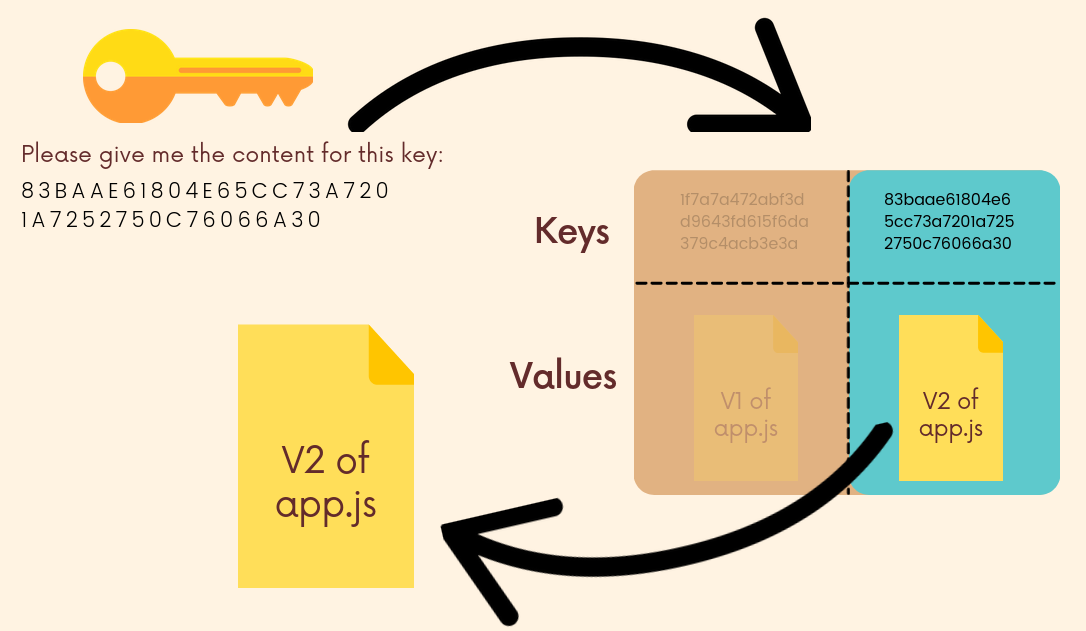
\includegraphics[width=3in]{screenshots/2022-07-10T15-18-37Z.png} 
\end{figure}

\section{Hashing With Git Hash-Objects}

\begin{tcolorbox}[title=Try Hashing,colback=backcolour]
\begin{lstlisting}[language=bash]
git hash-object <file>
# to take non-file input :
echo "hello" | git hash-object --stdin
# --stdin tells git to use the content from stdin rather than from a file
echo "hello" | git hash-object --stdin -w

# -w will add a file in .git/objects/??/hashfilename
\end{lstlisting}
\end{tcolorbox}

\section{Retrieving Data With Git Cat-File}

\begin{tcolorbox}[title=Retrieve Data,colback=backcolour]
\begin{lstlisting}[language=bash]
git cat-file -p <object-hash>
# -p tells git to pretty print the contents of the object based on its type
# works with 7-chars hashes too
git cat-file -p <object-hash> > filename.txt
\end{lstlisting}
\end{tcolorbox}

\section{Git Blobs}

\begin{itemize}
	\item Git blobs \textit{binary large object} are used to store the contents of files in a given repo. They don't include filenames, just raw content!
\end{itemize}

\section{Git Trees}

\begin{itemize}
	\item Git trees store structures, contents of a directory, contains pointers that can refer to blobs and other sub-trees 
	\item Each entry in a tree contains the SHA-1 hash of a blob or a tree aws mode, type and filename
\end{itemize}

\begin{figure}[H] 
	 \centering 
	 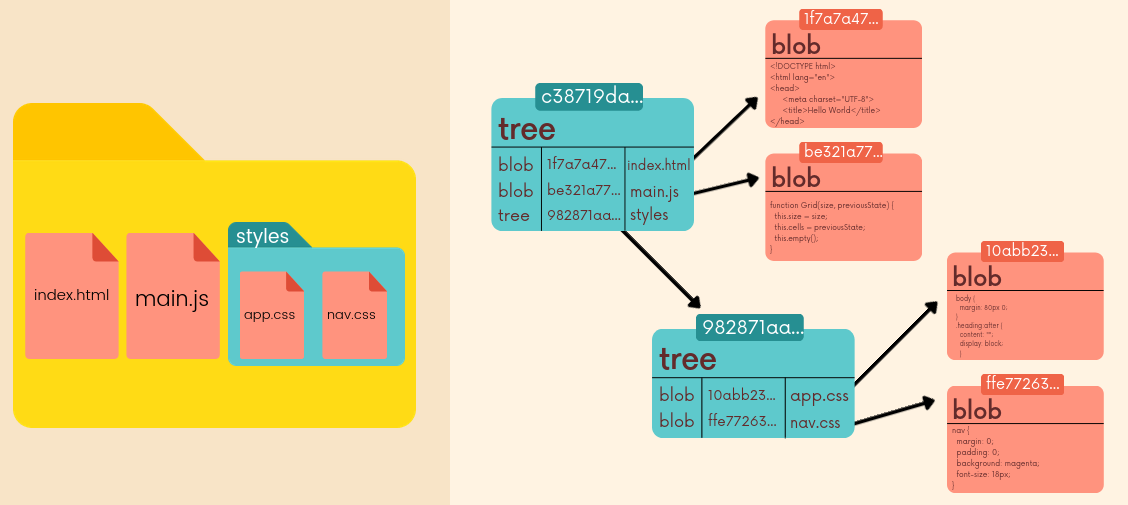
\includegraphics[width=4in]{screenshots/2022-07-10T17-18-43Z.png} 
\end{figure}

\begin{tcolorbox}[title=Viewing Trees,colback=backcolour]
\begin{lstlisting}[language=bash]
git cat-file -p master^{tree} 
# allows to view the tree that is here pointed to the tip of the master branch

git cat-file -t hash
# will give the type (blobs or tree)
\end{lstlisting}
\end{tcolorbox}

\section{Git Commits}

\begin{itemize}
	\item Commits objects combine a tree along with infos about the context that led to the current one. They sore refs to parents commit(s), author, commiter and message
\end{itemize}

\begin{figure}[H] 
	 \centering 
	 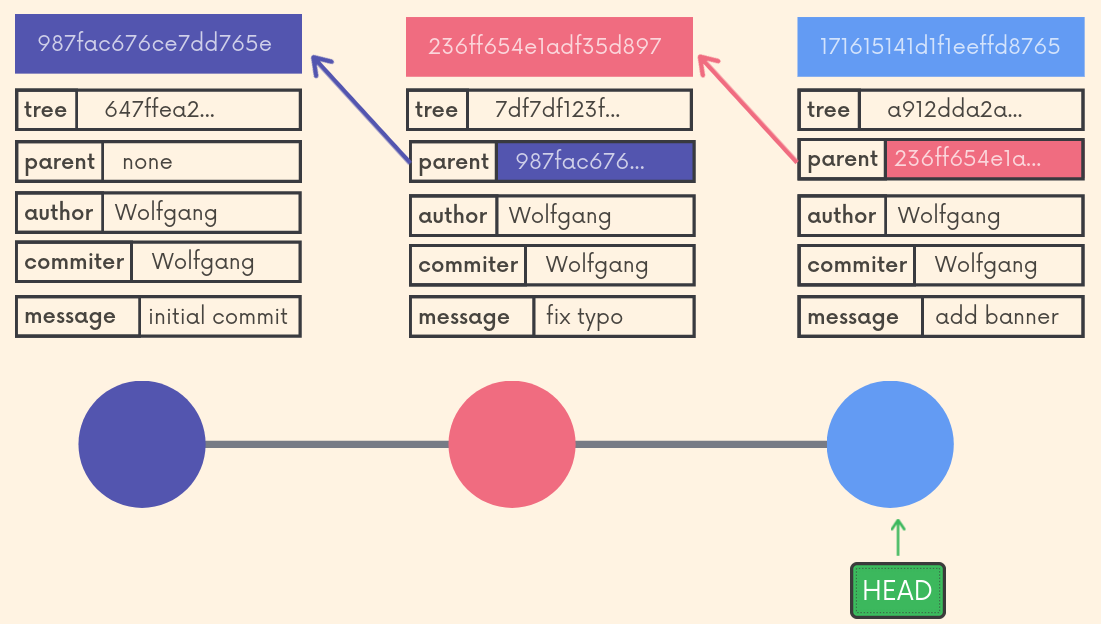
\includegraphics[width=2.7in]{screenshots/2022-07-10T18-43-56Z.png} 
	 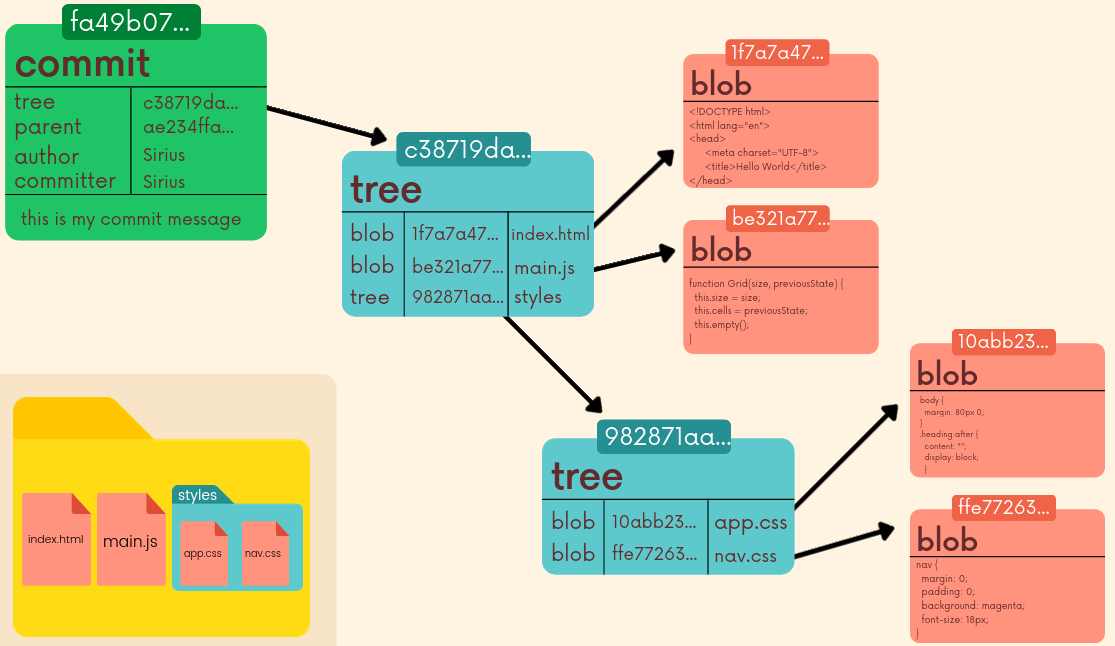
\includegraphics[width=2.7in]{screenshots/2022-07-10T18-43-14Z.png} 
\end{figure}


\chapter{The Power of Reflogs - Retreiving Lost Work}

\section{Introducing Reflogs}

\begin{itemize}
	\item \textbf{git reflogs} \textit{reference logs} keeps a record of when the tips of branches and other references were updated in the repo. Git is tracking our moves like branch switches, checkouts, is also tracking branches pointers
	\item the reflogs are kept in .git/logs/HEAD which is \textbf{readable}
\end{itemize}

\section{The Limitations Of Reflogs}

\begin{itemize}
	\item \warning reflogs are \textbf{only local} 
	\item Reflogs \textbf{expire} (after around 90 days by default) 
\end{itemize}

\section{Reflog Show Command}

\begin{itemize}
	\item \textbf{git reflog show HEAD} $\equiv$ \textbf{git show} : show is the default subcommand, it will show the log of a specific reference (defaults to HEAD) 
	\item we could also view logs for the tip of the main branch with \textbf{git reflog show main} 
\end{itemize}

\section{Reflog References}

\begin{itemize}
	\item We can access specific git refs in the form of \textbf{name@\{qualifier\}}. This syntax allows to access specific ref pointers and can pass them to other commands like checkout, reset and merge
	\item Reflog relative identifier in the form of HEAD@{i} or branch@{i} 
	\item Time-based \textbf{qualifier} fiters like 1.day.ago ; 3.minutes.ago ; yesterday ; Fri, 12 Feb 2021 14:06:21 -0800
\end{itemize}

\begin{tcolorbox}[title=Time-Based Examples,colback=backcolour]
\begin{lstlisting}[language=bash]
git reflog master@{one.week.ago}
git checkout bugfix@{2.days.ago}
git diff main@{0} main@{yesterday}
\end{lstlisting}
\end{tcolorbox}

\section{Reflogs Rescue}

\begin{tcolorbox}[title=Rescuing,colback=backcolour]
\begin{lstlisting}[language=bash]
git reset --hard hash1
# i want to undo removing hash1 commit
git reflog show master
git reset --hard master@{1}
# The new tip of the master branch becomes the lost hash1 commit, the commit is back !
\end{lstlisting}
\end{tcolorbox}

\section{Undoing A Rebase}

\begin{itemize}
	\item Rebasing \textbf{rewrittes} commits, so they appear to be gone
\end{itemize}

\begin{tcolorbox}[title=Example Of Undoing Rebase,colback=backcolour]
\begin{lstlisting}[language=bash]
git add file.txt
git commit -m "1"
git commit -am "2"
git switch -c "second"
git commit -am "3"
git commit -am "4"
git rebase -i HEAD~2
# proceeds to remove, fixup, reword
git reflog
# take the hash form a old commit
git reset --hard old_commit
# the rebasing is gone
\end{lstlisting}
\end{tcolorbox}


\chapter{Writing Custom Git Aliases}

\section{Global Git Config File}

\begin{itemize}
	\item Look either at \textbf{\$HOME/.gitconfig} or \textbf{\$HOME/.config/git/config}. Changes there will apply to every repos 
\end{itemize}

\begin{tcolorbox}[title=Adding Git Alias,colback=backcolour]
\begin{lstlisting}[language=bash]
[alias]
	s = status
	l = log
	ci = commit
\end{lstlisting}
\end{tcolorbox}

\begin{itemize}
	\item Setting aliases from the command line : \textbf{git config --global alias.whateveriwant branch} 
\end{itemize}

\begin{tcolorbox}[title=Aliases With Arguments,colback=backcolour]
\begin{lstlisting}[language=bash]
[alias]
	cm = commit -m
# anything put after will be appended
	a = add # file1 file2
\end{lstlisting}
\end{tcolorbox}

\begin{itemize}
	\item For existing good aliases, search online, example : \href{https://www.durdn.com/blog/2012/11/22/must-have-git-aliases-advanced-examples/}{\textbf{link1}} or, \href{https://github.com/GitAlias/gitalias}{\textbf{link2}}  
	\item \textbf{"!"} tells git that it is a shell script
\end{itemize}



\end{document}
